\subsection{User Study}\label{sec:user}

In this part, we conduct a comprehensive user study to evaluate the quality of visualizations generated by different methods.

\subsubsection{Settings}
We recruited ** participants with ** females, ** males, aged **-** with a mean of ** for the user study. The user study is conducted on the two larger datasets, i.e., \pt{} and \sz{}, and four methods are investigated, i.e., $\full$, $\rand$, $\mathsf{DTW}$ and $\avats$. We manually select 22 \textit{center points} in the two datasets and define 3 \textit{visualization scales} including:
large-scale region (zoom level less than 13), middle-scale region (zoom level between 13 and 15), small-scale region (zoom level more than 15). For each center point and visualization scale, we generate a \textit{comparable visualization group}, which includes one visualization generated by each of the 4 methods. This results in 66 comparable groups (22 center points $\times$ 3 scales) and 264 visualization results (66 comparable groups $\times$ 4 visualizations).

We are interested in the visual quality and visual clutter of the visualization results, and hence designed three tasks for a comparable group: \textit{T1}) rank the visualizations in the group from the highest visual quality to the lowest visual quality by 1-4;
\textit{T2}) rank the visualizations in the group from the least visual clutter to the most severe visual clutter by 1-4;
\textit{T3}) select the acceptable visualizations (multiple choices allowed) for analysis and choose the reason for those that are not selected, and we provide three reasons including ``severe visual clutter", ``poor visual quality" and ``others".  The user study system is a web-based platform, in which all visualizations are displayed with a resolution of 450*300.

\subsubsection{User study procedure}

When the participants enter the user study system, they are given a brief introduction and a tutorial on how to conduct the tasks to get familiar with the interface and tasks.
For each participant, we randomly select 16 comparable groups and generate 48 tasks.
For each comparable group, the 4 visualizations (\textit{without specifying generated by which method}) in one comparable group are shown on the same web-page and a participant is required to perform task T1, T2 and T3 by inspecting them.

%At last, the participants are interviewed to collect feedback after finishing the study and their answers are saved for result analysis.

\subsubsection{Result analysis}

\begin{figure*}[t]
	\centering
	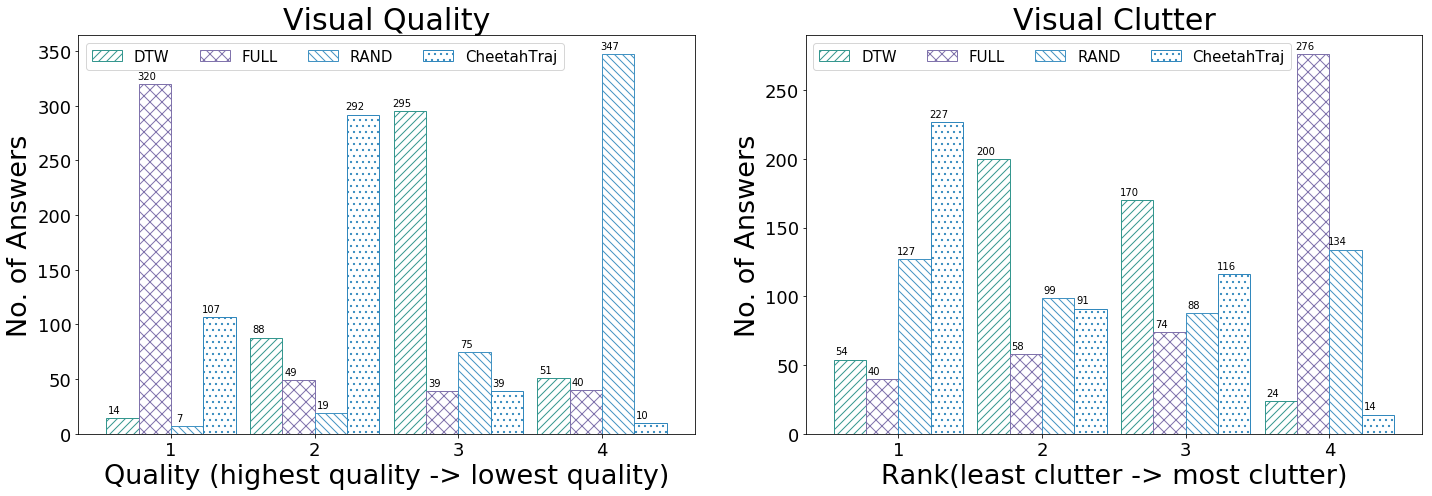
\includegraphics[width=0.6\textwidth]{pictures/user_study/rank.png}
	%\vspace{-3mm}
	\caption{User study, rank distribution.}
	\label{fig:rank}
	%\vspace{-2mm}
\end{figure*}

The left plot of Figure~\ref{fig:rank} reports the quality ranking of 4 methods in T1. The results show that $\full$ ranks the 1st in most cases while $\avats$ usually ranks 1st or 2nd. In contrast, $\mathsf{DTW}$ and $\rand$ rank 3rd and 4th in most cases. This suggests that $\avats$ outperforms $\mathsf{DTW}$ and $\rand$ in visual quality. We also found that $\avats$ ranks 1st mainly for large-scale regions in which there are many trajectories.         

 
%Figure~\ref{fig:rank} left shows the ranking among different methods with x-axis indicating the ranking from the highest quality to the lowest quality and y-axis indicating the selecting number for the specific method and ranking. The visualization of $\full$ has the highest visual quality since it has no information loss according the quality definition. The selection of $\avats$ is mostly concentrated at the first and second, which is closely behind the $\full$. The selections of $\baseline$ and $\rand$ are contracted at the third and fourth respectively, which is confirmed both of these two methods performs worse than $\full$ and $\qtavats$ in guarantee the visual quality.

The right plot of Figure~\ref{fig:rank} reports the anti-visual clutter ranking in T2. The results show that $\full$ has the most severe visual clutter, ranking 4th in most cases. $\rand$ and $\mathsf{DTW}$ reduce visual clutter via sampling, and thus usually rank 2nd and 3rd. $\avats$ is the most successful in reducing visual clutter, ranking 1st in 155 out of the xxx cases.       

%Figure~\ref{fig:rank} right reports the ranking among different methods with x-axis indicating the ranking from the least clutter to the most clutter and y-axis indicating the total selecting number for the specific method and ranking. We observe that the $\qtavats$ is ranked at the first 155 times which is significantly more than the other methods. The number it ranks at the second, third and last are 68, 96 and 14. There is no doubt that the visualization of $full$ suffers the most sever visual clutter problem because 210 of 333 total answers rank $full$ at the fourth, while other methods can be used to help to reduce the visual clutter.

We report the frequency each method is selected as acceptable and why a method is not selected for T3 using bar chart in Figure~\ref{fig:accept_rate}. Each column corresponds to a method and from left to right, the lengths of the bars means ``favorable'', ``not favorable due to visual clutter'', ``not favorable due to poor visual quality'' and ``not favorable for other reasons''. The results show that $\avats$ is acceptable in 85\% of the cases, and the other methods have significantly lower acceptance rate than $\avats$.      




\begin{figure}[t]
	\centering
	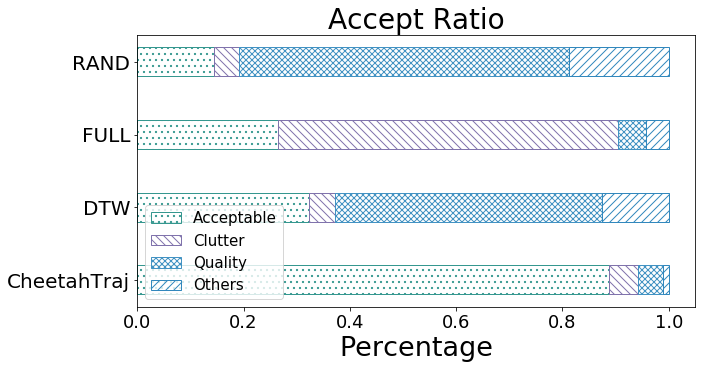
\includegraphics[width=0.35\textwidth]{pictures/user_study/accept_rate.png}
	%\vspace{-5mm}
	\caption{User study, accept rate.}
	\label{fig:accept_rate}
	%\vspace{-8mm}
\end{figure}





